\chapter{वायु, गैसों का एक मिश्रण}\label{ch:g4:air-a-mixture-of-gases}

\omterm{def:g4:air-a-mixture-of-gases:air}{हवा} वाले दिन पतंग अपनी डोर को खींचती है, और झील पर पाल \omterm{def:g4:air-a-mixture-of-gases:air}{हवा} से भरकर
नाव को आगे धकेलता है। कोई चीज़ उन्हें धकेल रही है, पर दिखाई कुछ नहीं
देता। वह चीज़ \omterm{def:g4:air-a-mixture-of-gases:air}{वायु} है। हम उसे देख नहीं सकते, पर वह हमारे चारों ओर है,
वह हर ख़ाली बोतल और हर कमरे को भरे रहती है, और हर साँस के साथ हम उसे
अंदर लेते हैं। \omterm{def:g4:air-a-mixture-of-gases:air}{वायु} किससे बनी है?

\begin{recall}
\omterm{def:g2:mixing-and-dissolving:mix}{मिलाना} यानी अलग-अलग चीज़ों को एक साथ रखना; जो मिलता है वह उन चीज़ों
का मिश्रण होता है, और मिलाने पर कुछ खोता नहीं
(\cref{ch:g2:mixing-and-dissolving})।
\end{recall}

\begin{omfigure}

\includegraphics[width=0.6\linewidth]{images/book1/ai/g4-kite-day.jpg}

{\small पतंग और पाल: \omterm{def:g4:air-a-mixture-of-gases:air}{वायु} दिखती नहीं, पर धकेलती है।}
\end{omfigure}

\section{वायु हमारे चारों ओर है}

\begin{example}[उलटा गिलास]\label{ex:g4:air-a-mixture-of-gases:glass}
एक सूखा काग़ज़ी रूमाल ख़ाली गिलास की तली तक ठूँस दिया जाता है। गिलास को
उलटा करके सीधे नीचे, पानी की एक कटोरी में दबाया जाता है। बाहर निकालने पर
रूमाल अब भी सूखा रहता है। गिलास ख़ाली नहीं था: वह \omterm{def:g4:air-a-mixture-of-gases:air}{वायु} से भरा था, और
\omterm{def:g4:air-a-mixture-of-gases:air}{वायु} ने पानी को अंदर नहीं आने दिया।
\end{example}

\begin{omfigure}
\begin{tikzpicture}[font=\small, scale=1.3]
  \pic[transform shape] at (0,0) {trough};
  % the upturned glass, rim at y = 0.35, base at y = 2.35
  \fill[white] (-0.8,0.5) rectangle (0.8,0.95);
  \pic[transform shape, rotate=180] at (0,2.35) {beaker={0}{white}};
  % the tissue at the top, inside
  \fill[white, draw=black!45, rounded corners=1.5pt] (-0.4,2.33) -- (-0.3,2.05)
    -- (-0.1,2.12) -- (0.05,1.98) -- (0.25,2.1) -- (0.42,2.02) -- (0.45,2.33) -- cycle;
  \draw[<-, omProp, thick] (0.45,2.12) -- (2.4,2.5) node[right, text=black]
    {सूखा रूमाल};
  \draw[<-, omProp, thick] (0.3,1.2) -- (2.4,1.4) node[right, text=black]
    {वायु: यह पानी को अंदर नहीं आने देती};
  \draw[<-, omProp, thick] (1.4,0.7) -- (2.4,0.55) node[right, text=black]
    {पानी};
\end{tikzpicture}

{\small गिलास को उलटा करके पानी में दबाया जाता है। अंदर फँसी \omterm{def:g4:air-a-mixture-of-gases:air}{वायु} पानी को
अंदर नहीं आने देती, और रूमाल सूखा रहता है।}
\end{omfigure}


\begin{remark}[वायु एक गैस है]\label{rem:g4:air-a-mixture-of-gases:gas}
\omterm{def:g4:air-a-mixture-of-gases:air}{वायु} एक गैस है: उसका अपना कोई आकार नहीं होता और वह फैलकर किसी भी बर्तन
को भर देती है। फिर भी वह द्रव्य है, और \omterm{def:g4:air-a-mixture-of-gases:air}{वायु} से भरा गुब्बारा उसी ख़ाली
गुब्बारे से थोड़ा भारी होता है। गैसें क्या हैं, और वे ऐसा व्यवहार क्यों
करती हैं, यह भौतिकी की पुस्तक में बताया गया है।
\end{remark}

\section{वायु एक मिश्रण है}

\begin{definition}[वायु]\label{def:g4:air-a-mixture-of-gases:air}
\emph{वायु}\index{वायु} गैसों का वह मिश्रण है जो पृथ्वी को घेरे हुए है।
वह कोई एक अकेली गैस नहीं है: उसमें कई गैसें मिली हुई हैं, और उन्हें
एक-दूसरे से अलग किया जा सकता है।
\end{definition}

\begin{proposition}[वायु किससे बनी है]\label{prop:g4:air-a-mixture-of-gases:composition}
% ledger: air:N2, air:O2, air:Ar, air:trace, air:CO2, air:H2O
जलवाष्प को छोड़ दें, तो \omterm{def:g4:air-a-mixture-of-gases:air}{वायु} इनसे बनी है:
\begin{itemize}
  \item \textbf{नाइट्रोजन}, \omterm{def:g4:air-a-mixture-of-gases:air}{वायु} का लगभग चार-पाँचवाँ भाग;
  \item \textbf{ऑक्सीजन}, \omterm{def:g4:air-a-mixture-of-gases:air}{वायु} का लगभग पाँचवाँ भाग;
  \item थोड़ी-सी \textbf{आर्गन}, लगभग 100 में 1 भाग;
  \item बहुत थोड़ी-सी \textbf{कार्बन डाइऑक्साइड}, लगभग 10\,000 में 4 भाग,
        और दूसरी गैसों की बहुत छोटी-छोटी मात्राएँ।
\end{itemize}
\omterm{def:g4:air-a-mixture-of-gases:air}{वायु} में अदृश्य \textbf{जलवाष्प} भी होती है: सूखे, ठंडे दिन बहुत कम,
और गरम, नम दिन 100 में लगभग 4 भाग तक।
\end{proposition}

\begin{example}[वायु की सौ बोतलें]\label{ex:g4:air-a-mixture-of-gases:hundred}
% ledger: air:N2, air:O2, air:Ar
सूखी \omterm{def:g4:air-a-mixture-of-gases:air}{वायु} की 100 बोतलों की कल्पना करो, और मान लो कि \omterm{def:g4:air-a-mixture-of-gases:air}{वायु} की गैसों को
अलग-अलग बोतलों में छाँट दिया गया है। लगभग 78 बोतलों में नाइट्रोजन होगी,
21 बोतलों में ऑक्सीजन, और आख़िरी बोतल में आर्गन, साथ में कुछ बूँदों भर
कार्बन डाइऑक्साइड और दूसरी गैसें।
\end{example}

\begin{omfigure}
\begin{tikzpicture}[font=\small, x=0.42cm, y=0.42cm]
  \foreach \k in {0,...,99} {
    \pgfmathtruncatemacro\col{mod(\k,10)}
    \pgfmathtruncatemacro\row{9-int(\k/10)}
    \ifnum\k<78 \def\c{omDef!45}\else\ifnum\k<99 \def\c{red!45}\else\def\c{cyan!60}\fi\fi
    \fill[\c, draw=white, line width=0.8pt] (\col,\row) rectangle ++(1,1);
  }
  \fill[omDef!45] (12,8) rectangle ++(1,1);
  \node[anchor=west] at (13.3,8.5) {नाइट्रोजन: 78 वर्ग};
  \fill[red!45] (12,6) rectangle ++(1,1);
  \node[anchor=west] at (13.3,6.5) {ऑक्सीजन: 21 वर्ग};
  \fill[cyan!60] (12,4) rectangle ++(1,1);
  \node[anchor=west, align=left] at (13.3,4.5) {आर्गन, कार्बन डाइऑक्साइड\\ और बाकी: 1 वर्ग};
\end{tikzpicture}

{\small सूखी \omterm{def:g4:air-a-mixture-of-gases:air}{वायु} के सौ वर्ग। नीचे दाईं ओर के वर्ग में आर्गन है, और वह
कार्बन डाइऑक्साइड भी, जो अलग से बनाने के लिए बहुत कम है।}
\end{omfigure}

\begin{remark}[गैसों के नाम]\label{rem:g4:air-a-mixture-of-gases:names}
नाइट्रोजन, ऑक्सीजन, आर्गन और कार्बन डाइऑक्साइड गैसों के नाम हैं। ये
सभी रंगहीन हैं और इनमें कोई गंध नहीं होती। आगे का एक अध्याय दिखाता है
कि इनमें से हर एक किससे बनी है, उन नन्हे कणों तक जिनसे सारा द्रव्य बना है।
\end{remark}

\section{हम कौन-सी वायु अंदर लेते और बाहर छोड़ते हैं}

\begin{proposition}[छोड़ी हुई साँस की वायु]\label{prop:g4:air-a-mixture-of-gases:breath}
% ledger: breath:O2, breath:CO2, breath:N2, air:O2, air:CO2
जो \omterm{def:g4:air-a-mixture-of-gases:air}{वायु} हम बाहर छोड़ते हैं, वह वही नहीं है जो हमने अंदर ली थी। हमारा
शरीर कुछ ऑक्सीजन ले लेता है और कार्बन डाइऑक्साइड और जलवाष्प बाहर देता है:
\begin{itemize}
  \item अंदर ली गई \omterm{def:g4:air-a-mixture-of-gases:air}{वायु} के 100 में लगभग 21 भाग ऑक्सीजन होते हैं, पर
        बाहर छोड़ी गई \omterm{def:g4:air-a-mixture-of-gases:air}{वायु} के 100 में केवल लगभग 16 भाग;
  \item कार्बन डाइऑक्साइड 10\,000 में लगभग 4 भाग से बढ़कर 100 में लगभग 4
        भाग हो जाती है: लगभग सौ गुना;
  \item नाइट्रोजन जितनी अंदर ली जाती है, उतनी ही बाहर छोड़ी जाती है।
\end{itemize}
\end{proposition}

\begin{omfigure}
\begin{tikzpicture}
\begin{axis}[ybar, width=0.8\linewidth, height=5.2cm, bar width=12pt,
    ymin=0, ymax=90, ylabel={100 में भाग},
    symbolic x coords={nitrogen, oxygen, carbon dioxide}, xtick=data,
    xticklabels={नाइट्रोजन, ऑक्सीजन, कार्बन डाइऑक्साइड},
    tick label style={font=\small}, label style={font=\small},
    xticklabel style={text height=1.6ex, text depth=0.4ex},
    legend style={font=\small, at={(0.98,0.95)}, anchor=north east},
    nodes near coords, nodes near coords style={font=\footnotesize},
    enlarge x limits=0.25, axis lines*=left, ymajorgrids,
    grid style={gray!20}]
% ledger: air:N2, air:O2, air:CO2, breath:N2, breath:O2, breath:CO2 (rounded)
\addplot[fill=omDef!45, draw=omDef] coordinates
  {(nitrogen,78) (oxygen,21) (carbon dioxide,0)};
\addplot[fill=omProp!55, draw=omProp] coordinates
  {(nitrogen,78) (oxygen,16) (carbon dioxide,4)};
\legend{अंदर ली गई, बाहर छोड़ी गई}
\end{axis}
\end{tikzpicture}

{\small अंदर ली गई और बाहर छोड़ी गई \omterm{def:g4:air-a-mixture-of-gases:air}{वायु}, 100 में भागों में (जलवाष्प छोड़कर,
संख्याएँ पूर्णांकित)। अंदर ली गई \omterm{def:g4:air-a-mixture-of-gases:air}{वायु} की कार्बन डाइऑक्साइड, 10\,000 में
4 भाग, इतनी कम है कि उसे दंड के रूप में नहीं दिखाया जा सकता।}
\end{omfigure}

\begin{example}[भरा हुआ कमरा]\label{ex:g4:air-a-mixture-of-gases:room}
खिड़कियाँ बंद किए एक छोटी कक्षा में तीस लोग पूरी सुबह कार्बन डाइऑक्साइड
बाहर छोड़ते हैं। धीरे-धीरे कमरे की \omterm{def:g4:air-a-mixture-of-gases:air}{वायु} में ऑक्सीजन घटती जाती है और
कार्बन डाइऑक्साइड बढ़ती जाती है, और लोग थकान महसूस करते हैं। खिड़कियाँ
खोलने से ताज़ी \omterm{def:g4:air-a-mixture-of-gases:air}{वायु} फिर अंदर आ जाती है।
\end{example}

\begin{omfigure}
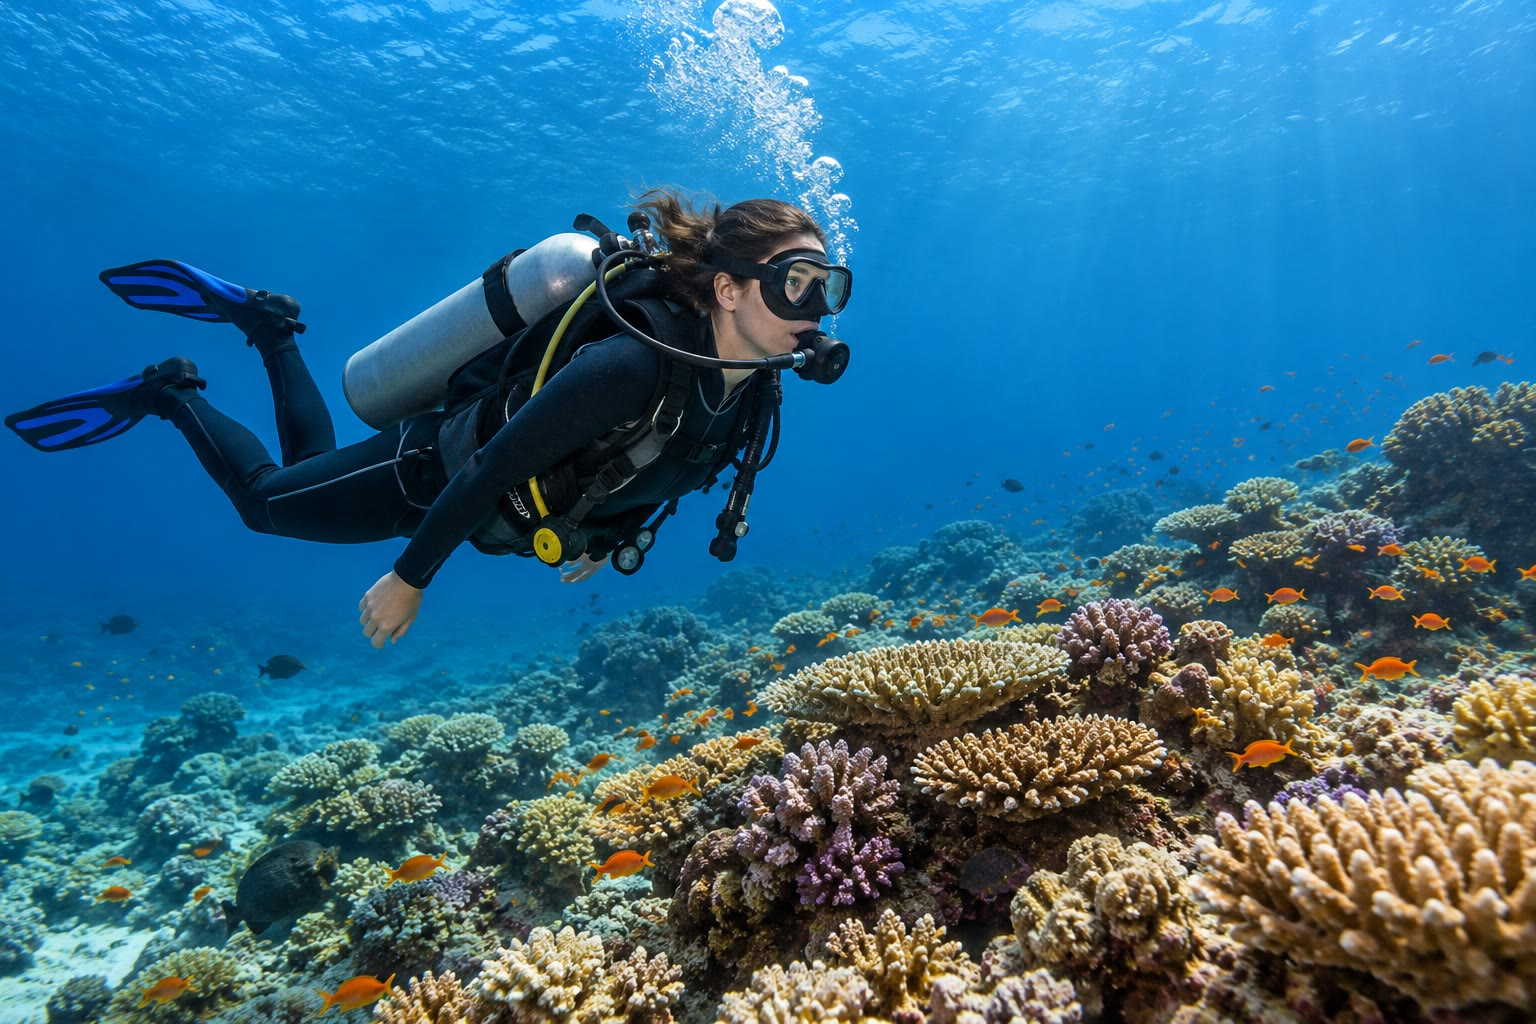
\includegraphics[width=0.55\linewidth]{images/book1/ai/g4-scuba-diver.jpg}

{\small गोताख़ोर पीठ पर लगे सिलिंडर से \omterm{def:g4:air-a-mixture-of-gases:air}{वायु} लेता है; बुलबुले उसकी बाहर
छोड़ी हुई \omterm{def:g4:air-a-mixture-of-gases:air}{वायु} हैं।}
\end{omfigure}

\begin{remark}[गोताख़ोर वायु क्यों लेते हैं]\label{rem:g4:air-a-mixture-of-gases:diver}
गोताख़ोर के सिलिंडर में शुद्ध ऑक्सीजन नहीं, बल्कि छोटी-सी जगह में दबाकर
भरी गई \omterm{def:g4:air-a-mixture-of-gases:air}{वायु} होती है: पानी में गहरे जाकर शुद्ध ऑक्सीजन लेना ख़तरनाक है।
\omterm{def:g4:air-a-mixture-of-gases:air}{वायु} की नाइट्रोजन ऑक्सीजन को हल्का करने के लिए होती है।
\end{remark}

\section{जीवन और आग के लिए ऑक्सीजन}

\begin{proposition}[सजीव और लौ ऑक्सीजन की खपत करते हैं]\label{prop:g4:air-a-mixture-of-gases:oxygen}
\omterm{def:g4:air-a-mixture-of-gases:air}{वायु} की सारी गैसों में से ऑक्सीजन ही वह गैस है जिसकी सजीवों और लौ को
ज़रूरत होती है। जंतु और मनुष्य साँस लेते समय उसे अंदर लेते हैं; लौ उसे
अपने आस-पास की \omterm{def:g4:air-a-mixture-of-gases:air}{वायु} से लेती है। हरे पौधे दिन के उजाले में ऑक्सीजन वापस
\omterm{def:g4:air-a-mixture-of-gases:air}{वायु} में छोड़ते हैं।
\end{proposition}

\begin{inthelab}[मर्तबान के नीचे मोमबत्ती]
शिक्षक एक टाइल पर मोमबत्ती जलाते हैं और उस पर काँच का एक बड़ा मर्तबान
धीरे-धीरे उलटा रख देते हैं। लौ छोटी होती है, टिमटिमाती है और कुछ सेकंड
बाद बुझ जाती है: लौ के आस-पास की \omterm{def:g4:air-a-mixture-of-gases:air}{वायु} में उसे जलाए रखने लायक ऑक्सीजन
नहीं बची। दुगने बड़े मर्तबान के नीचे मोमबत्ती लगभग दुगने समय तक जलती है,
क्योंकि वहाँ लगभग दुगनी \omterm{def:g4:air-a-mixture-of-gases:air}{वायु} है, और इसलिए खपत के लिए दुगनी
ऑक्सीजन।
\end{inthelab}

\begin{omfigure}
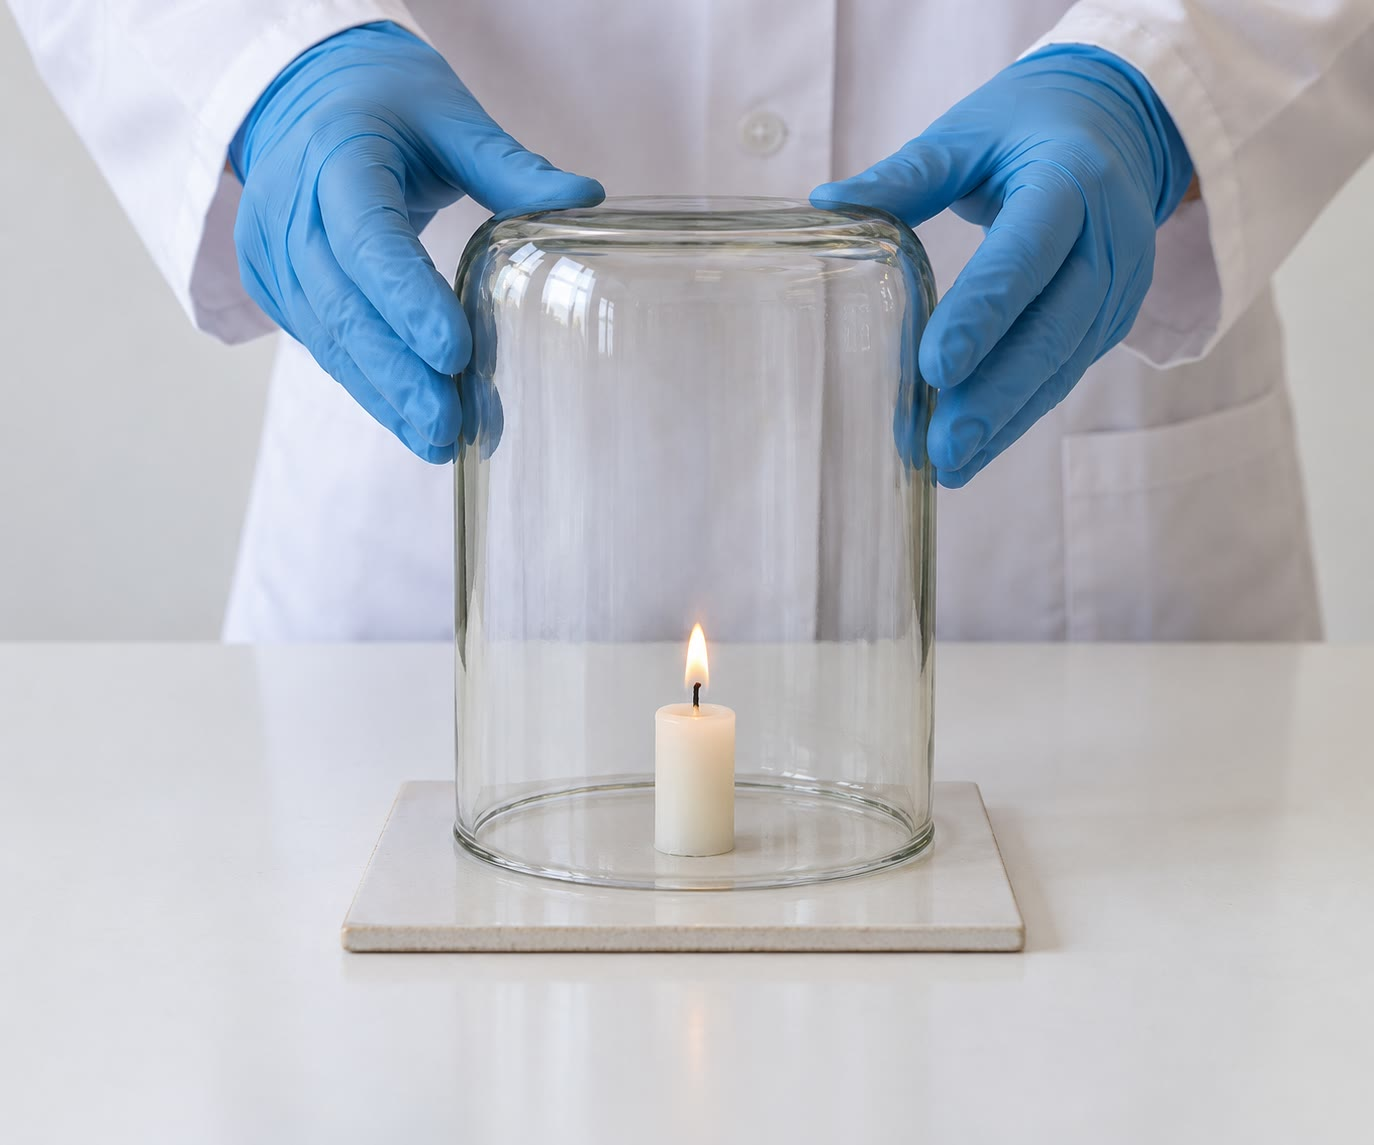
\includegraphics[width=0.5\linewidth]{images/book1/ai/g4-candle-jar-lab.jpg}

{\small काँच के मर्तबान के नीचे मोमबत्ती तब बुझ जाती है जब उसकी लौ के
आस-पास बहुत कम ऑक्सीजन बचती है।}
\end{omfigure}

\begin{remark}[नाइट्रोजन नहीं जलती]\label{rem:g4:air-a-mixture-of-gases:nitrogen}
नाइट्रोजन \omterm{def:g4:air-a-mixture-of-gases:air}{वायु} का सबसे बड़ा भाग है, फिर भी वह लौ को जलाए नहीं रखती और
हमारा शरीर उसका उपयोग नहीं करता। अगर \omterm{def:g4:air-a-mixture-of-gases:air}{वायु} पूरी की पूरी नाइट्रोजन होती,
तो हम साँस नहीं ले पाते और कुछ भी नहीं जल पाता।
\end{remark}

\section{अभ्यास}

\begin{exercise}[$\star$]\label{exo:g4:air-a-mixture-of-gases:1}
क्या \omterm{def:g4:air-a-mixture-of-gases:air}{वायु} एक अकेली गैस है या एक मिश्रण? \omterm{def:g4:air-a-mixture-of-gases:air}{वायु} की दो मुख्य गैसों के नाम बताओ।
\end{exercise}

\begin{exercise}[$\star$]\label{exo:g4:air-a-mixture-of-gases:2}
\omterm{def:g4:air-a-mixture-of-gases:air}{वायु} का लगभग कितना भाग नाइट्रोजन है? लगभग कितना भाग
ऑक्सीजन है?
\end{exercise}

\begin{exercise}[$\star$]\label{exo:g4:air-a-mixture-of-gases:3}
सूखी \omterm{def:g4:air-a-mixture-of-gases:air}{वायु} के 100 लीटर में लगभग कितने लीटर नाइट्रोजन है? लगभग कितने
लीटर ऑक्सीजन है?
\end{exercise}

\begin{exercise}[$\star$]\label{exo:g4:air-a-mixture-of-gases:4}
एक ख़ाली बोतल को उलटा करके पानी के टब में डाला जाता है। पानी बोतल को
क्यों नहीं भर देता?
\end{exercise}

\begin{exercise}[$\star$]\label{exo:g4:air-a-mixture-of-gases:5}
दंड-आरेख देखो। बाहर छोड़ी गई \omterm{def:g4:air-a-mixture-of-gases:air}{वायु} में कौन-सी गैस कम है? कौन-सी गैस
ज़्यादा है?
\end{exercise}

\begin{exercise}[$\star$]\label{exo:g4:air-a-mixture-of-gases:6}
लौ को \omterm{def:g4:air-a-mixture-of-gases:air}{वायु} की कौन-सी गैस चाहिए? साँस लेते समय हमें \omterm{def:g4:air-a-mixture-of-gases:air}{वायु} की कौन-सी गैस
चाहिए?
\end{exercise}

\begin{exercise}[$\star$]\label{exo:g4:air-a-mixture-of-gases:7}
100 वर्गों वाला चित्र देखो। कितने वर्ग नाइट्रोजन हैं? कितने
नाइट्रोजन नहीं हैं?
\end{exercise}

\begin{exercise}[$\star$]\label{exo:g4:air-a-mixture-of-gases:8}
मर्तबान के नीचे रखी मोमबत्ती कुछ देर बाद क्यों बुझ जाती है?
\end{exercise}

\begin{exercise}[$\star$]\label{exo:g4:air-a-mixture-of-gases:9}
500 लीटर \omterm{def:g4:air-a-mixture-of-gases:air}{वायु} में लगभग कितने लीटर ऑक्सीजन है? (\omterm{def:g4:air-a-mixture-of-gases:air}{वायु} का पाँचवाँ भाग
ऑक्सीजन है।)
\end{exercise}

\begin{exercise}[$\star\star$]\label{exo:g4:air-a-mixture-of-gases:10}
दो कक्षाओं के बीच में कक्षा की खिड़कियाँ खोलना अच्छा क्यों है?
\end{exercise}

\begin{exercise}[$\star\star$]\label{exo:g4:air-a-mixture-of-gases:11}
एक छोटे मर्तबान के नीचे मोमबत्ती 10 सेकंड तक जलती है। तिगुनी \omterm{def:g4:air-a-mixture-of-gases:air}{वायु} वाले
मर्तबान के नीचे वह लगभग कितनी देर जलेगी?
\end{exercise}
